\item Buzz-Status module
	
The Buzz-Status module was expected to at least implement these 6 functional processes:
	
\begin{enumerate}
	\item assessProfile:
	\begin{itemize}
		\item\textbf{Objective: } Serve as a general interface through which lecturers can choose a pluggable implementation with which to assess user profiles.
		\item\textbf{Pre-conditions: } Have some form of administrative and general users. Have profiles for users of the Buzz system. 
		\item\textbf{Post-conditions: } ProfileAssessor can return queried information about a users profile according to various criteria but must, as a minimal requirement, at least be able to calculate the user’s status (i.e. the user’s rating).
		\item\textbf{Testing: } Although both pre-conditions were met, no actual implementation for this functional requirement is present in the Buzz system (meaning post-conditions not met).
	\end{itemize}
\item setStatusCalculator:
	\begin{itemize}
		\item\textbf{Objective: } An interface through which a StatusCalculator can be assigned. The StatusCalculator is used to assign a status value to a user according to specific criteria. The default StatusCalculator should be NumPostAssesor which assigns a status directly proportional to the number of posts a user has made.
		\item\textbf{Pre-conditions: } Have some form of administrative and general users. Have profiles for users of the Buzz system. Have a space where users can post content (this is a pre-condition for the default StatusCalculator, i.e. NumPostAssessor).
		\item\textbf{Post-conditions: } The assigned StatusCalculator must be able to assign a status value to all users.
		\item\textbf{Testing: } Only the first two pre-conditions are met. Although there is a space where users can post content (i.e. http://buzz-codechat.rhcloud.com/spaces/) it does not fulfil any of its required functionality (i.e. can’t successfully post content, no thread handling). There is no implementation of a StatusCalculator present in the Buzz system, therefore no post-conditions were met.
	\end{itemize}
\item getStatusForProfile:
	\begin{itemize}
		\item\textbf{Objective: } A simple query which returns the user’s status.
		\item\textbf{Pre-conditions: } Have profiles for users of the Buzz system. Each user has a status.
		\item\textbf{Post-conditions: } The user’s status is returned.
		\item\textbf{Testing: } Only the first pre-condition is met (i.e. user’s do not have statuses). There is no way of storing a user’s status in the Buzz system, it therefore fails to meet the post-condition.
	\end{itemize}
\item createAppraisalType:
	\begin{itemize}
		\item\textbf{Objective: }  Be able to create a data structure by which posts can be graded/appraised (e.g. FunnyAppraisalType allows user to mark a post as Hilarious, Funny or Boring).
		\item\textbf{Pre-conditions: } Have a space were posts can be displayed.
		\item\textbf{Post-conditions: }Have a user created data structure which can then be used to appraise/rank a post.
		\item\textbf{Testing: } The pre-condition is not met as although a space for posts exists, none of the required functionality exist (e.g. being able to post new content in a thread). The post-conditions are not met as no functions in the Buzz system implements the required functionality.
	\end{itemize}
\item activateAppraisalType:
	\begin{itemize}
		\item\textbf{Objective: } Assign an appraisal type (which was created by createAppraisalType) to be used in a specific Buzz space for a specific period of time.
		\item\textbf{Pre-conditions: }  Have a space were posts can be displayed. Have a function(s) which implements createAppraisalType.
		\item\textbf{Post-conditions: }Be able to use user created appraisal types in a certain buzz space for a specific period of time.
		\item\textbf{Testing: }  Neither pre-conditions are met as the Buzz space does not function properly and no version of createAppraisalType was implemented. This function was not implemented which means no post-conditions were met.
\begin{figure}[h!]
  \centering
    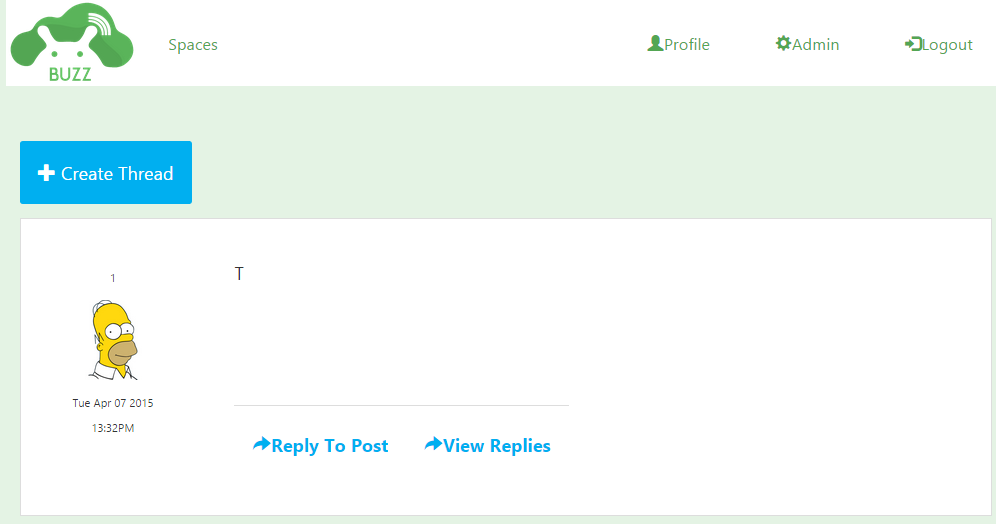
\includegraphics[width=0.85\textwidth]{No_appraisal}
    \caption{There are no appraisal icons with which to "upvote" posts}
\end{figure}	
	\end{itemize}
\item assignAppraisalToPost:
	\begin{itemize}
		\item\textbf{Objective: } Allows the user to assign an appraisal to a post (i.e. rate a post).
		\item\textbf{Pre-conditions: }  Have a space were posts can be displayed.
		\item\textbf{Post-conditions: }The ranking/status of both the post and the user who posted the post will change.
		\item\textbf{Testing: } The pre-condition is not met as  the Buzz space does not function properly. This function was not implemented which means no post-conditions were met.
	\end{itemize}
\end{enumerate}